\documentclass[journal=jpcbfk]{achemso}

\usepackage[version=3]{mhchem}
\usepackage[T1]{fontenc}
\newcommand*\mycommand[1]{\texttt{\emph{#1}}}
\newcommand{\todo}[1]{\textcolor{red}{#1}}

\usepackage{upgreek}				
\usepackage{xcolor}
\usepackage{booktabs}
\usepackage{multirow}
\usepackage{lmodern}
\usepackage{microtype}
\usepackage{xr}
\externaldocument{manuscriptPS}

\author{Pavel Buslaev}
\affiliation{Moscow Institute of Physics and Technology}
\author{Tiago M. Ferreira}
\affiliation{Halle, Germany}
\author{Ivan Gushchin}
\affiliation{Moscow Institute of Physics and Technology}
\author{Matti Javanainen}
\affiliation{Institute of Organic Chemistry and Biochemistry,
Academy of Sciences of the Czech Republic, 
Prague 6, Czech Republic}
\author{Batuhan Kav}
\affiliation{Potsdam, Germany}
\author{Jesper J. Madsen}
\affiliation{Department of Chemistry, The University of Chicago, Chicago, Illinois 60637, United States of America}
\author{Markus Miettinen}
\affiliation{Potsdam, Germany}
\author{Josef Melcr}
\affiliation{Institute of Organic Chemistry and Biochemistry,
Academy of Sciences of the Czech Republic, 
Prague 6, Czech Republic}
\author{Ricky Nencini}
\affiliation{Institute of Organic Chemistry and Biochemistry,
Academy of Sciences of the Czech Republic, 
Prague 6, Czech Republic}
\author{O. H. Samuli Ollila}
\email{samuli.ollila@helsinki.fi}
%\homepage[]{Your web page}
\affiliation{Institute of Organic Chemistry and Biochemistry,
Academy of Sciences of the Czech Republic, 
Prague 6, Czech Republic}
\affiliation{Institute of Biotechnology, University of Helsinki}
\author{Thomas Piggot   \todo{Authorlist is not yet complete}}
\affiliation{Southampton, United Kingdom}






\SectionNumbersOn

\renewcommand{\thetable}{S\arabic{table}}%
\renewcommand{\thefigure}{S\arabic{figure}}%
\renewcommand{\thesection}{S\arabic{section}}%
\renewcommand{\thepage}{S\arabic{page}}%

\title{ Supporting Information:\\ NMRlipids IV: Headgroup \& glycerol backbone structures, and cation binding in bilayers with PS lipids}

\begin{document}

\newpage
%\tableofcontents

\section{Simulated systems}

\subsection{CHARMM36}
\todo{To be written by Piggot, Madsen and Ollila}

\subsection{CHARMM36ua}
\todo{To be written by Piggot}

\subsection{Slipids}
\todo{To be written by Piggot and Favela}

\subsection{Berger}
\todo{To be written by Piggot and Ollila}
Simulations with excess sodium were taken directly from Ref. \citenum{jurkiewicz12} and
simulations with calcium directly from \citenum{melcrova16}.
Simulation of POPC at 310 K was taken directly from Ref. \citenum{ollila07a}.

\subsection{GROMOS-CKP}
\todo{To be written by Piggot}
  CKPM refers to the version with Berger/Chiu NH$_3$ charges compatible with Berger
   (i.e. the NH$_3$ group having the same charges as in the N(CH$_3$)$_3$ group of the PC lipids;
   'M' stands for Mukhopadhyay after the first published Berger-based PS simulation that used these charges~\cite{mukhopadhyay04})
   and CKP refers to the version with more Gromos compatible version
   (i.e. the charges for the NH$_3$ group taken from the lysine side-chain).

\subsection{Lipid17}
\todo{To be written by Kav, Miettinen and Meclr.}

\subsection{MacRog}
\todo{To be written by Javanainen and Piggot}


\section{Electrometer concept in PC lipid bilayers mixed with negatively charged lipids}\label{electrometerFORmixtures}

The electrometer concept is based on the empirical observations that
the order parameters of $\alpha$ and $\beta$ carbons in PC lipid headgroup
decrease (increase) proportionally to the bound positive (negative) 
charge~\cite{akutsu81,altenbach84,seelig87,scherer89} (Fig. \ref{HGorderparametersPCvsPEPSPGchol}). 
Therefore, the headgroup order parameters can be used to measure the
ion binding affinity to lipid bilayers containing PC
lipids~\cite{akutsu81,altenbach84,borle85,seelig87,macdonald87,roux90}.
Changes of the headgroup order parameters of other lipids with bound charge,
like negatively charged PS and PG lipids,  are also systematic,
but less well characterized~\cite{borle85,macdonald87,roux86,roux90}.
Therefore, the ion binding affinity to negatively charged bilayers
can be better characterized measuring the PC headgroup order parameters from 
mixed bilayers~\cite{borle85,roux86,macdonald87,roux90,roux91}.
\begin{figure}[]
  \centering
  \includegraphics[width=8.0cm]{../Figs/HGorderparametersPCvsPEPSPGchol.eps}
  \caption{\label{HGorderparametersPCvsPEPSPGchol}
    Headgroup order parameters of POPC measured from mixtures with
    PS (bovine brain), POPG, POPE, cholesterol and cationic dihexadecyldimethylammonium bromide (DHAB) surfactant~\cite{scherer87,scherer89,ferreira13}.
    Signs are taken from separate experiments~\cite{ollila16,ferreira16}.
  }
\end{figure}

When comparing ion binding measured from the PC headgroup order parameters between
neutral and anionic membranes, it is important to note that the order parameters
increase due to the addition of negative charged lipids according to the electrometer
concept~\cite{seelig87, scherer87} (Fig. \ref{HGorderparametersPCvsPEPSPGchol}).
Therefore, the headgroup order parameters of POPC in mixtures with anionic
lipids are larger than in pure POPC lipid bilayer, which is also seen in the ion binding
experiments from different mixtures in the absence of added calcium (Fig. \ref{OrderParametersWithCaCl}).
Upon addition of CaCl$_2$, the order parameters decrease and reach the values of pure PC bilayer close 
to the CaCl$_2$ concentrations of $\sim$ 50-300mM, depending on the amount of negatively charged
lipids in the mixture (Fig. \ref{OrderParametersWithCaCl}).
Around these concentrations the positive charge of bound Ca$^{2+}$ cancels
the negative charge lipids, resulting to a neutral membrane. 
Above such concentrations, the specific binding of calcium leads to
the overcharging of the membrane.
\begin{figure}[]
  \centering
  \includegraphics[width=8.0cm]{../Figs/LIPIDSwithCaCl.eps}
  \includegraphics[width=8.0cm]{../Figs/LIPIDSwithCaClBELOW1M.eps}
  \caption{\label{OrderParametersWithCaCl}
    Headgroup order parameters of POPC as a function of CaCl concentration from experiments 
    different mole fractions of negatively charged lipids (left column).
    Right column shows the same data zoomed to the concentrations below 1M.
    Data for Pure DPPC from~\cite{akutsu81},
    for pure POPC from~\cite{altenbach84}, 
    for POPC:POPS (5:1) mixture from~\cite{roux90},
    for POPC:POPG (8:2,1:1) mixtures with 0.1M NaCl from~\cite{macdonald87}
    and for POPC:POPG (1:1) mixture data without NaCl from \cite{borle85}.
  }
\end{figure}

Because the POPC headgroup order parameters in mixtures with different amounts of anionic lipids
but without additional salt are not equal, the binding affinity of calcium can be better compared
by plotting the changes of order parameters as a function of added calcium.
As expected, such a plot reveals more pronounced order parameter decrease in systems
with larger fractions of negatively charged lipids (Fig. \ref{OrderParameterCHANGESWithCaClBELOW1M}),
indicating an increase in the calcium binding affinity with the increasing amount of negatively charged
lipids in membranes. In conclusion, the presented empirical comparison of headgroup order parameter changes
from various mixtures of POPC and anionic lipids with added calcium gives physically
consistent results, suggesting that the electrometer concept can be used to determine
the cation binding affinity also to the lipid bilayers containing mixtures of PC and anionic lipids.  
\begin{figure}[]
  \centering
  \includegraphics[width=9.0cm]{../Figs/CHANGESwithCaCl.eps}
  \caption{\label{OrderParameterCHANGESWithCaClBELOW1M}
    Changes of POPC headgroup order parameters as a function of CaCl$_2$
    measured from mixed bilayers containing different amounts of anionic lipids.
    The original data is the same as in figure~\ref{OrderParametersWithCaCl}.
%    The values are taken from 2H NMR experiments reported in the
%    literature (DPPC \cite{akutsu81}, POPC \cite{altenbach84}, POPC:POPS (5:1) \cite{roux90},
%    POPC:POPG  mixtures with 0.1M NaCl \cite{macdonald87}
%    and POPC:POPG (1:1) without NaCl \cite{borle85}).
  }
\end{figure}

\pagebreak
\section{Calibration of PC headgroup order parameter response to the bound cations}\label{electrometerCALIBRATION}
Before using the headgroup order parameters to compare ion binding affinity between simulations
and experiments, the response of the order parameters to the bound charge in simulations should be quantified
against experiments~\cite{catte16,melcr18}. In our previous work~\cite{catte16},
the ratio $\Delta S_{\rm CH}^\beta / \Delta S_{\rm CH}^\alpha$ was in good agreement with the experiments~\cite{akutsu81}
in the Lipid14 model, but was underestimated by other models. In the more recent study~\cite{melcr18},
the headgroup order parameter responses were compared more carefully with the experiments of
cationic dihexadecyldimethylammonium bromide (DHAB) surfactants in POPC bilayer~\cite{scherer89}.
The comparison reveals that the both headgroup order parameters in the Lipid14 model are too sensitive to the bound charge,
while CHARMM36 gives better agreement for the $\alpha$ carbon (Fig. \ref{CHANGESwithDHMDMAB}).
Therefore, the headgroup order parameter response to the bound charge is actually more realistic
in CHARMM36 model than in the Lipid14. In the latter, both order parameters are equally too 
sensitive to the bound cations giving a good result for the $\Delta S_{\rm CH}^\beta / \Delta S_{\rm CH}^\alpha$ ratio.
The ratio was overestimated for the CHARMM36 model because the $\beta$-carbon order parameter
is relatively more sensitive than the $\alpha$-carbon order parameter. These results have to be taken
into account when analysing the ion binding affinities using headgroup order parameters in simulations.
However, we conclude that the discrepancies arising from the sentivity of lipid headgroup to
bound charge are typically smaller than then discrepancies arising from ion binding affinity.
\begin{figure}[]
  \centering
  \includegraphics[width=9.0cm]{../Figs/HGopsDHMDMAB.eps}
  \caption{\label{CHANGESwithDHMDMAB}
  Responses of headgroup order parameters to the fixed amount of cationic surfactants in
  POPC bilayer from simulations and experiments \cite{scherer89}.
  The simulation results for Lipid14 are directly from Ref.~\citenum{melcr18}.
  The CHARMM36 simulation data and details are available from Ref.~\citenum{CHARMM36cationicSURF}.
}
\end{figure}

\pagebreak
\section{Effect of the definition of concentration on the headgroup order parameters as a function of ion concentration.}\label{concentrationDEFsection}
Previous studies using the electrometer concept to assess the ion binding affinity to lipid
bilayers report ion concentrations either in water before solvating the lipids \cite{akutsu81,roux90,catte16}
or in bulk water after solvating the lipids \cite{altenbach84,melcr18}.
In this work, we use the former definition to be consistent with the reference
experimental data \cite{roux90}. The difference between these two concentrations increases
with the increasing ion binding affinity. However, the difference is essentially negligible
in the recent model \cite{melcr18} with realistic ion binding affinity (Fig. \ref{concentrationDEFfigure}).
\begin{figure}[]
  \centering
  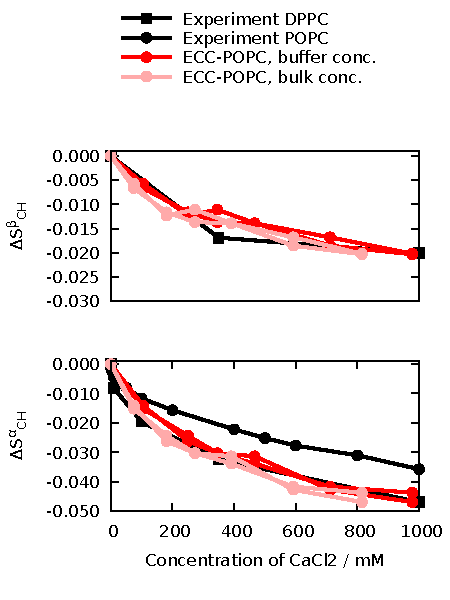
\includegraphics[width=9.0cm]{../Figs/OP_ECC_POPC_DPPC_water_conc2_dppc_bulk.pdf}
  \caption{\label{concentrationDEFfigure}
    Difference between order parameter changes as a function of CaCl$_2$ concentration demonstrated
    for the two possible definitions of ion concentration, concentration in buffer before solvating the
    lipids (buffer concentration) and concentration in bulk after solvating the lipids (bulk concentration),
    from the recent model with realistic calcium binding affinity to a POPC bilayer \cite{melcr18}. 
}
\end{figure}

\pagebreak
\section{Dipolar slices of the R-PDFL experiment}

Slices of the R-PDFL spectra (Fig. \ref{DPslices}) 
show a single splitting for the $\beta$-carbon with the order parameter value of 0.12,
and a superposition of a large and a very small splitting for the $\alpha$-carbon.
The larger splitting gives a order parameter value of 0.09, while the numerical value
from the small splitting cannot resolved with the available resolution.
\begin{figure}[]
%  \centering
  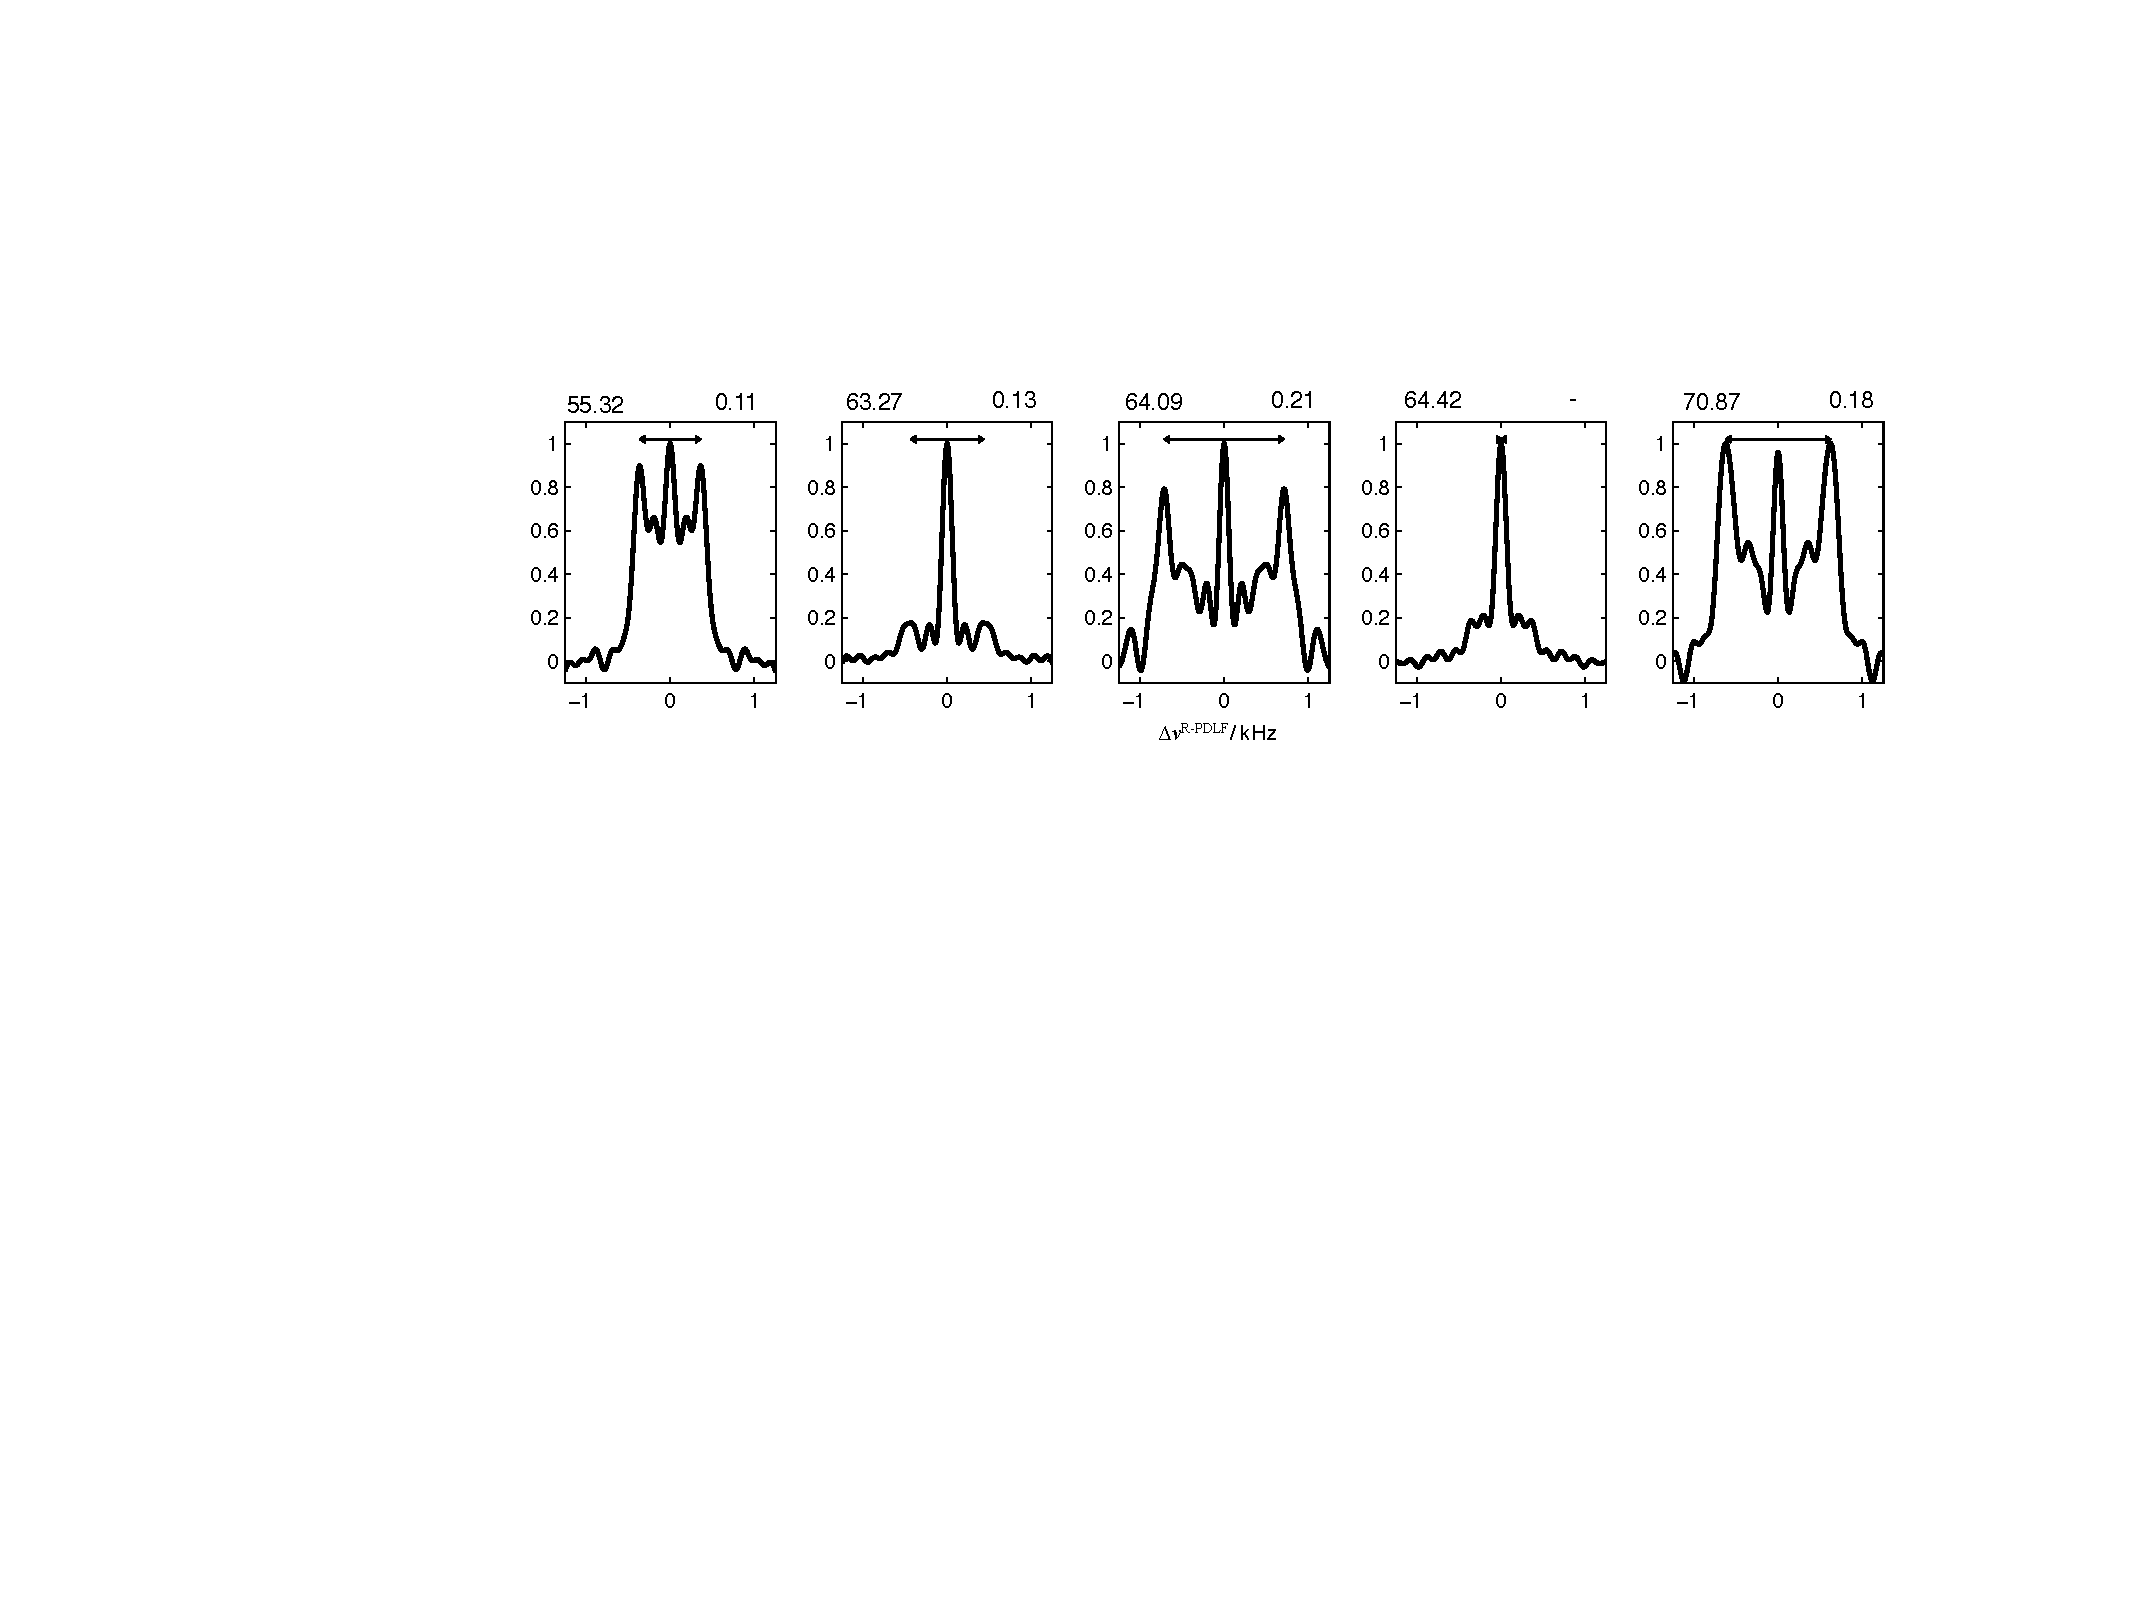
\includegraphics[width=20.0cm]{../Figs/SI_slices.pdf}
  \caption{\label{DPslices}
    Dipolar coupling slices from the R-PDFL experiment.
  }
  \todo{Labeling of carbons and explanations of numbers (chemical shift and order parameter) would be good.
  Also, the size of the figure in the file may not be optimal.}
\end{figure}

\pagebreak
\section{Dihedral angle distributions of the headgroup and glycerol backbone
  regions of PS lipids from different simulation models}

The glycerol backbone order parameters of C$_2$ and C$_3$ from Slipids simulations
differ significantly from the other simulation results and experiments (Fig. \ref{HGorderParametersPS}),
as observed previously also for PC lipids \cite{botan15}.
The origin of this difference is more difficult to track without more elaborate analysis,
because different models show very complicated patterns of distinct structures
in the glycerol backbone region (Figs.~\ref{HGstructuresPS} and \ref{dihedralsHG}).

\begin{figure*}[]
  \centering
  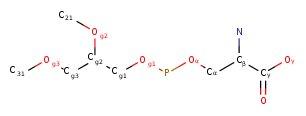
\includegraphics[width=8.0cm]{../Figs/PS_Labels.png}
  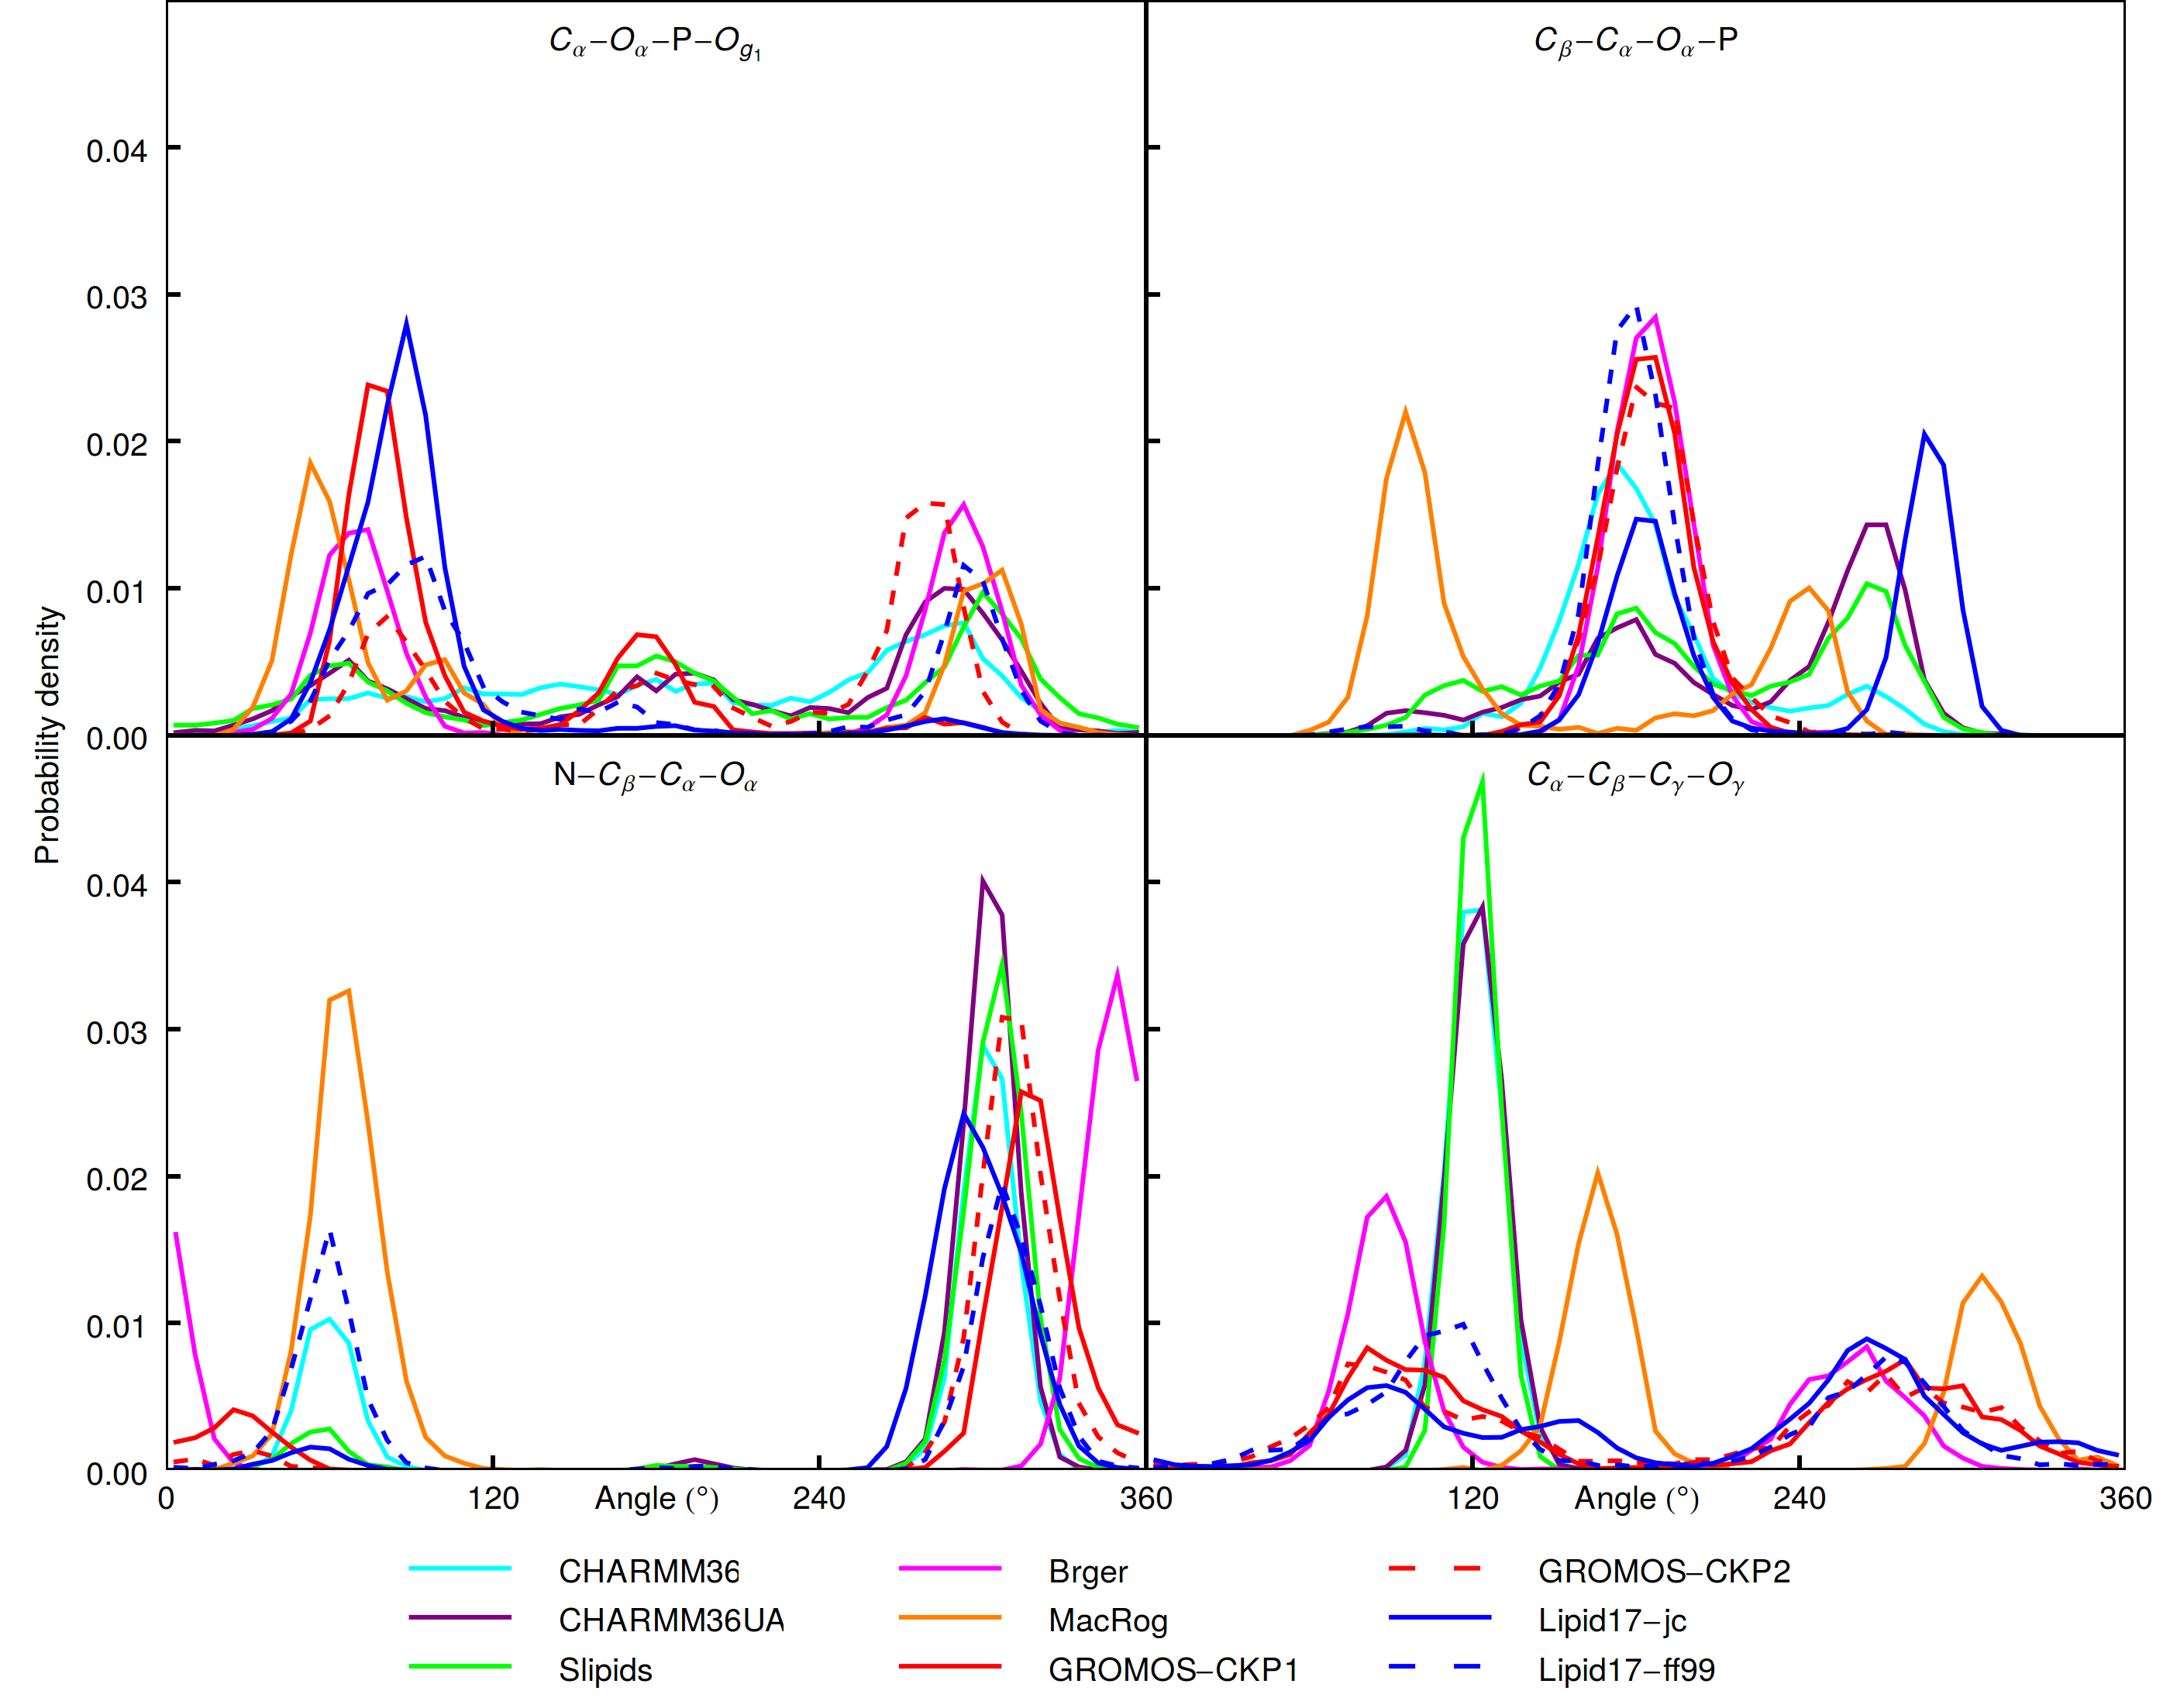
\includegraphics[width=16.0cm]{../Figs/figS7.png}
  \caption{\label{dihedralsHG}
    Dihedral angle distributions of headgroup region of PS lipids from different simulation models.
  }
\end{figure*}

\begin{figure*}[]
  \centering
  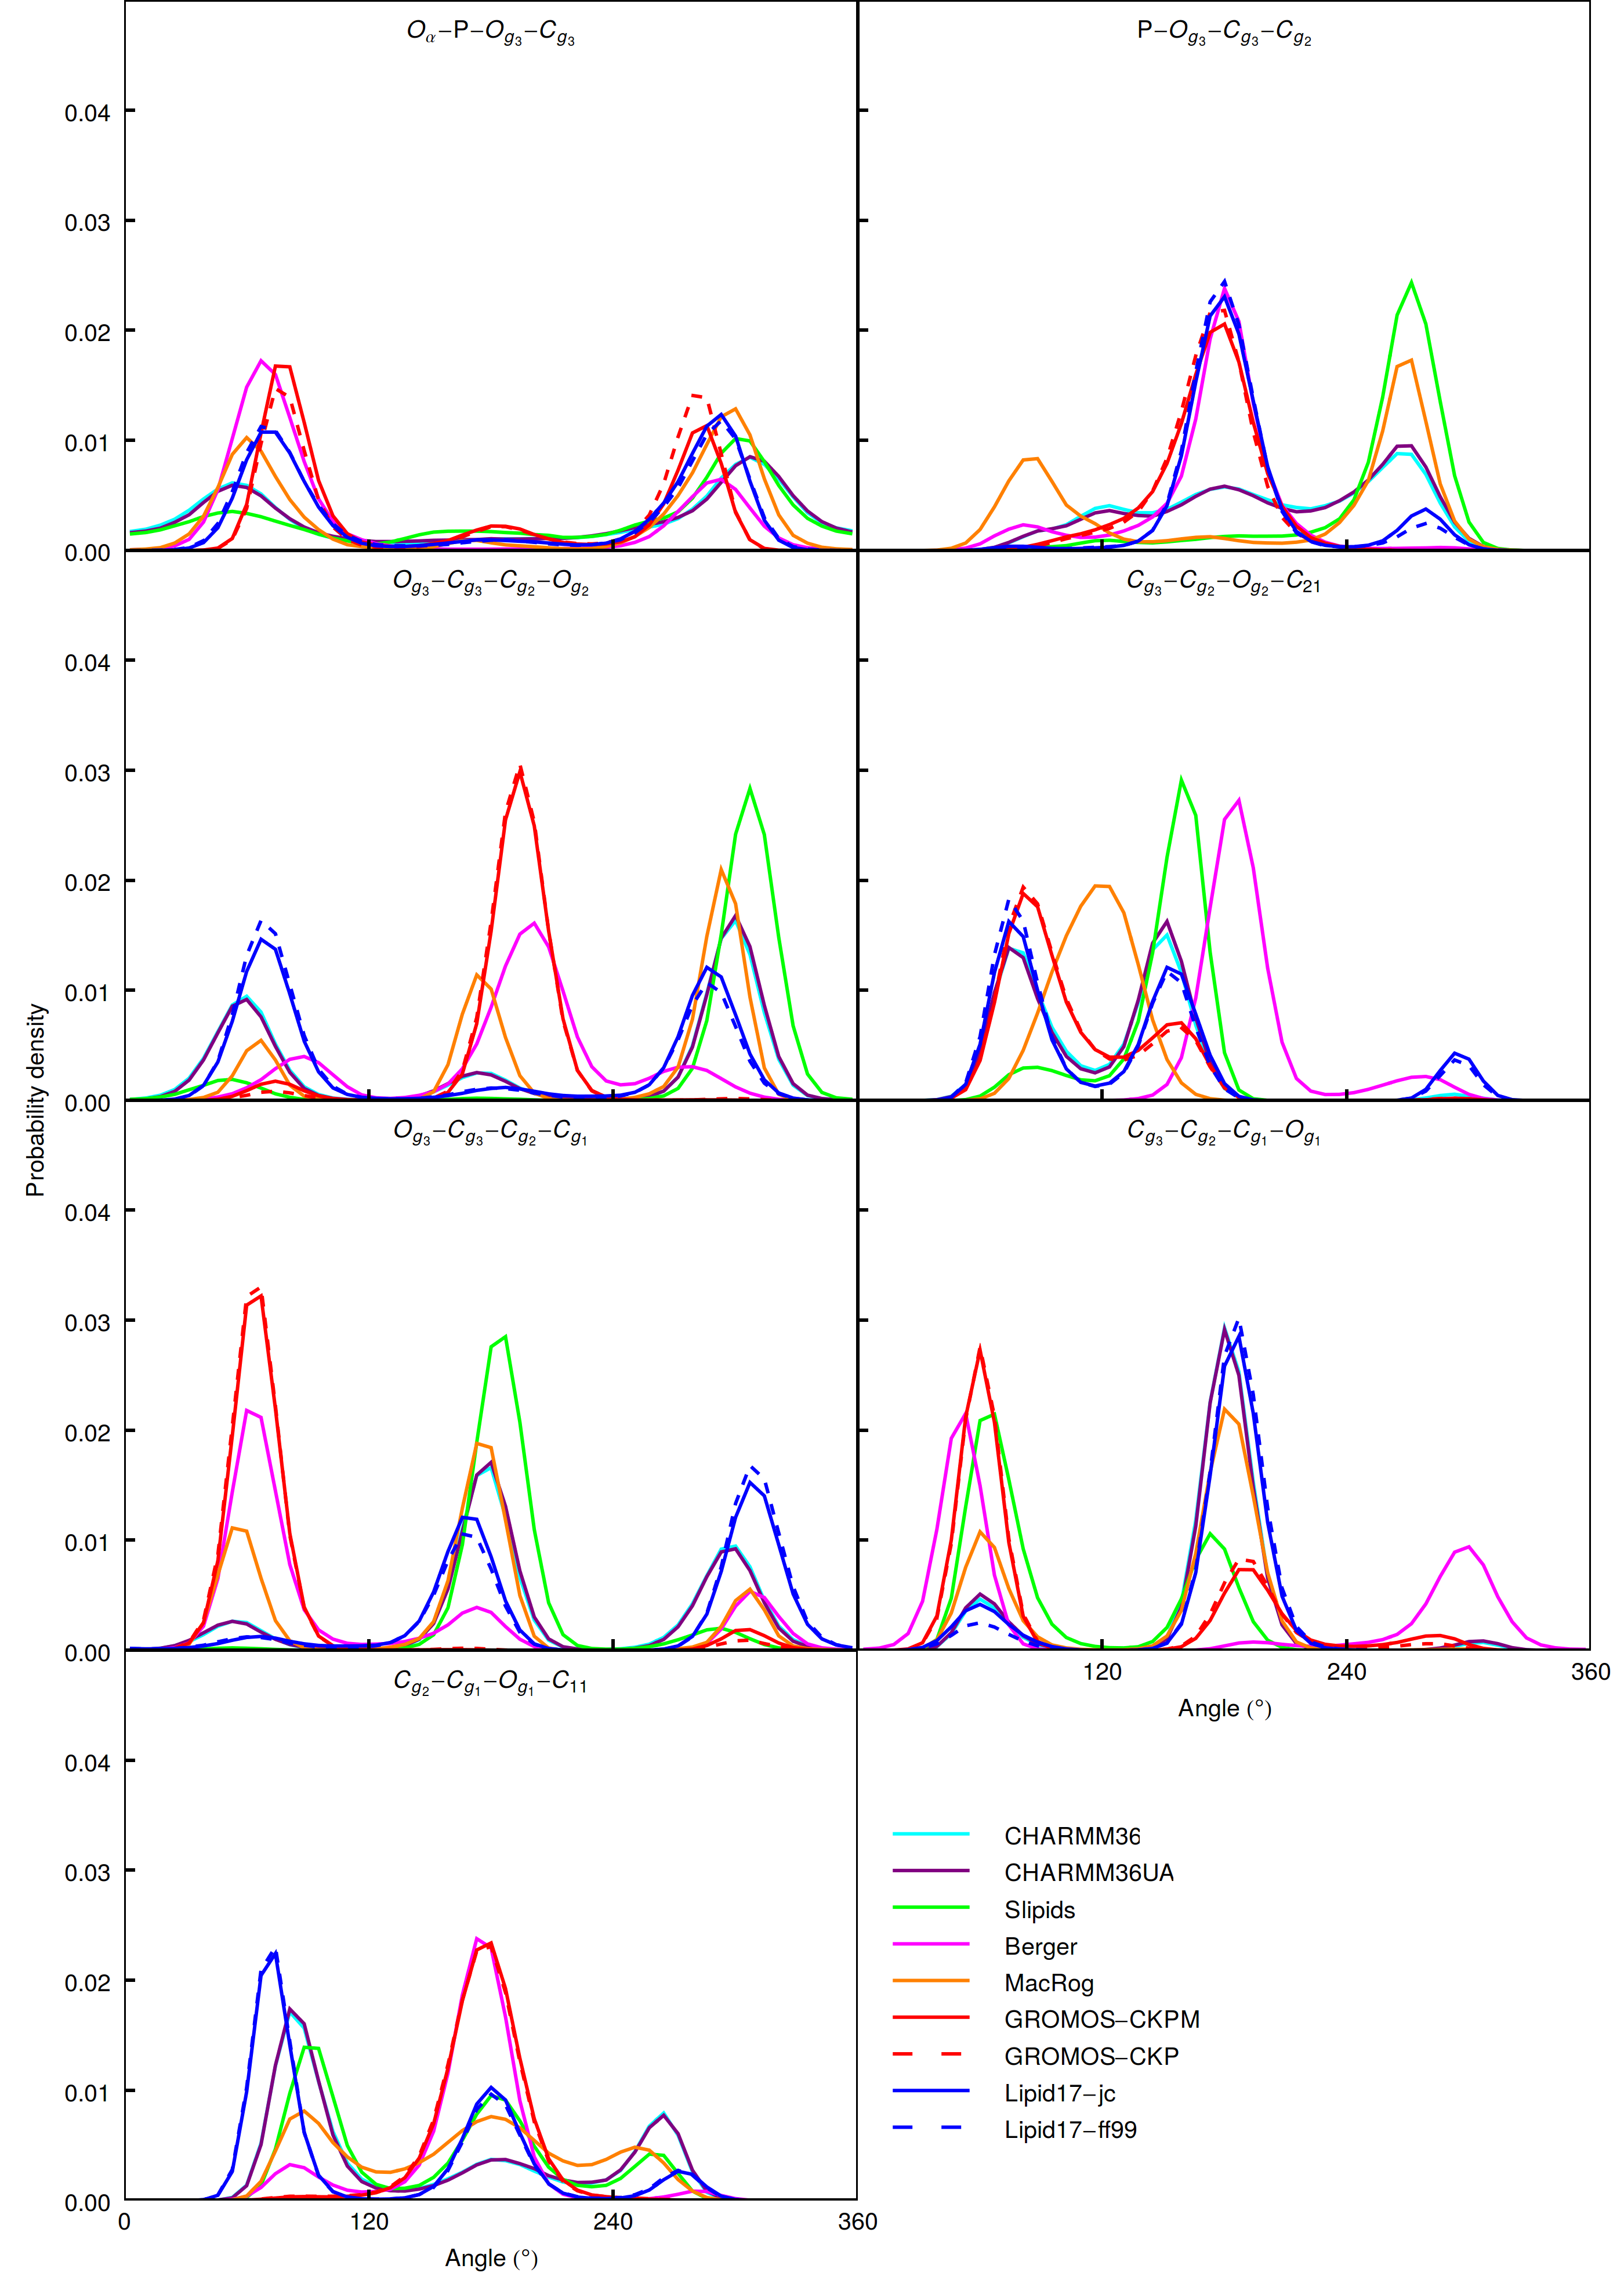
\includegraphics[width=15.0cm]{../Figs/figS6.png}
  \caption{\label{dihedralsGLY}
    Dihedral angle distributions of glycerol backbone region of PS lipids from different simulation models.
  }
\end{figure*}

\begin{figure*}[]
  \centering
  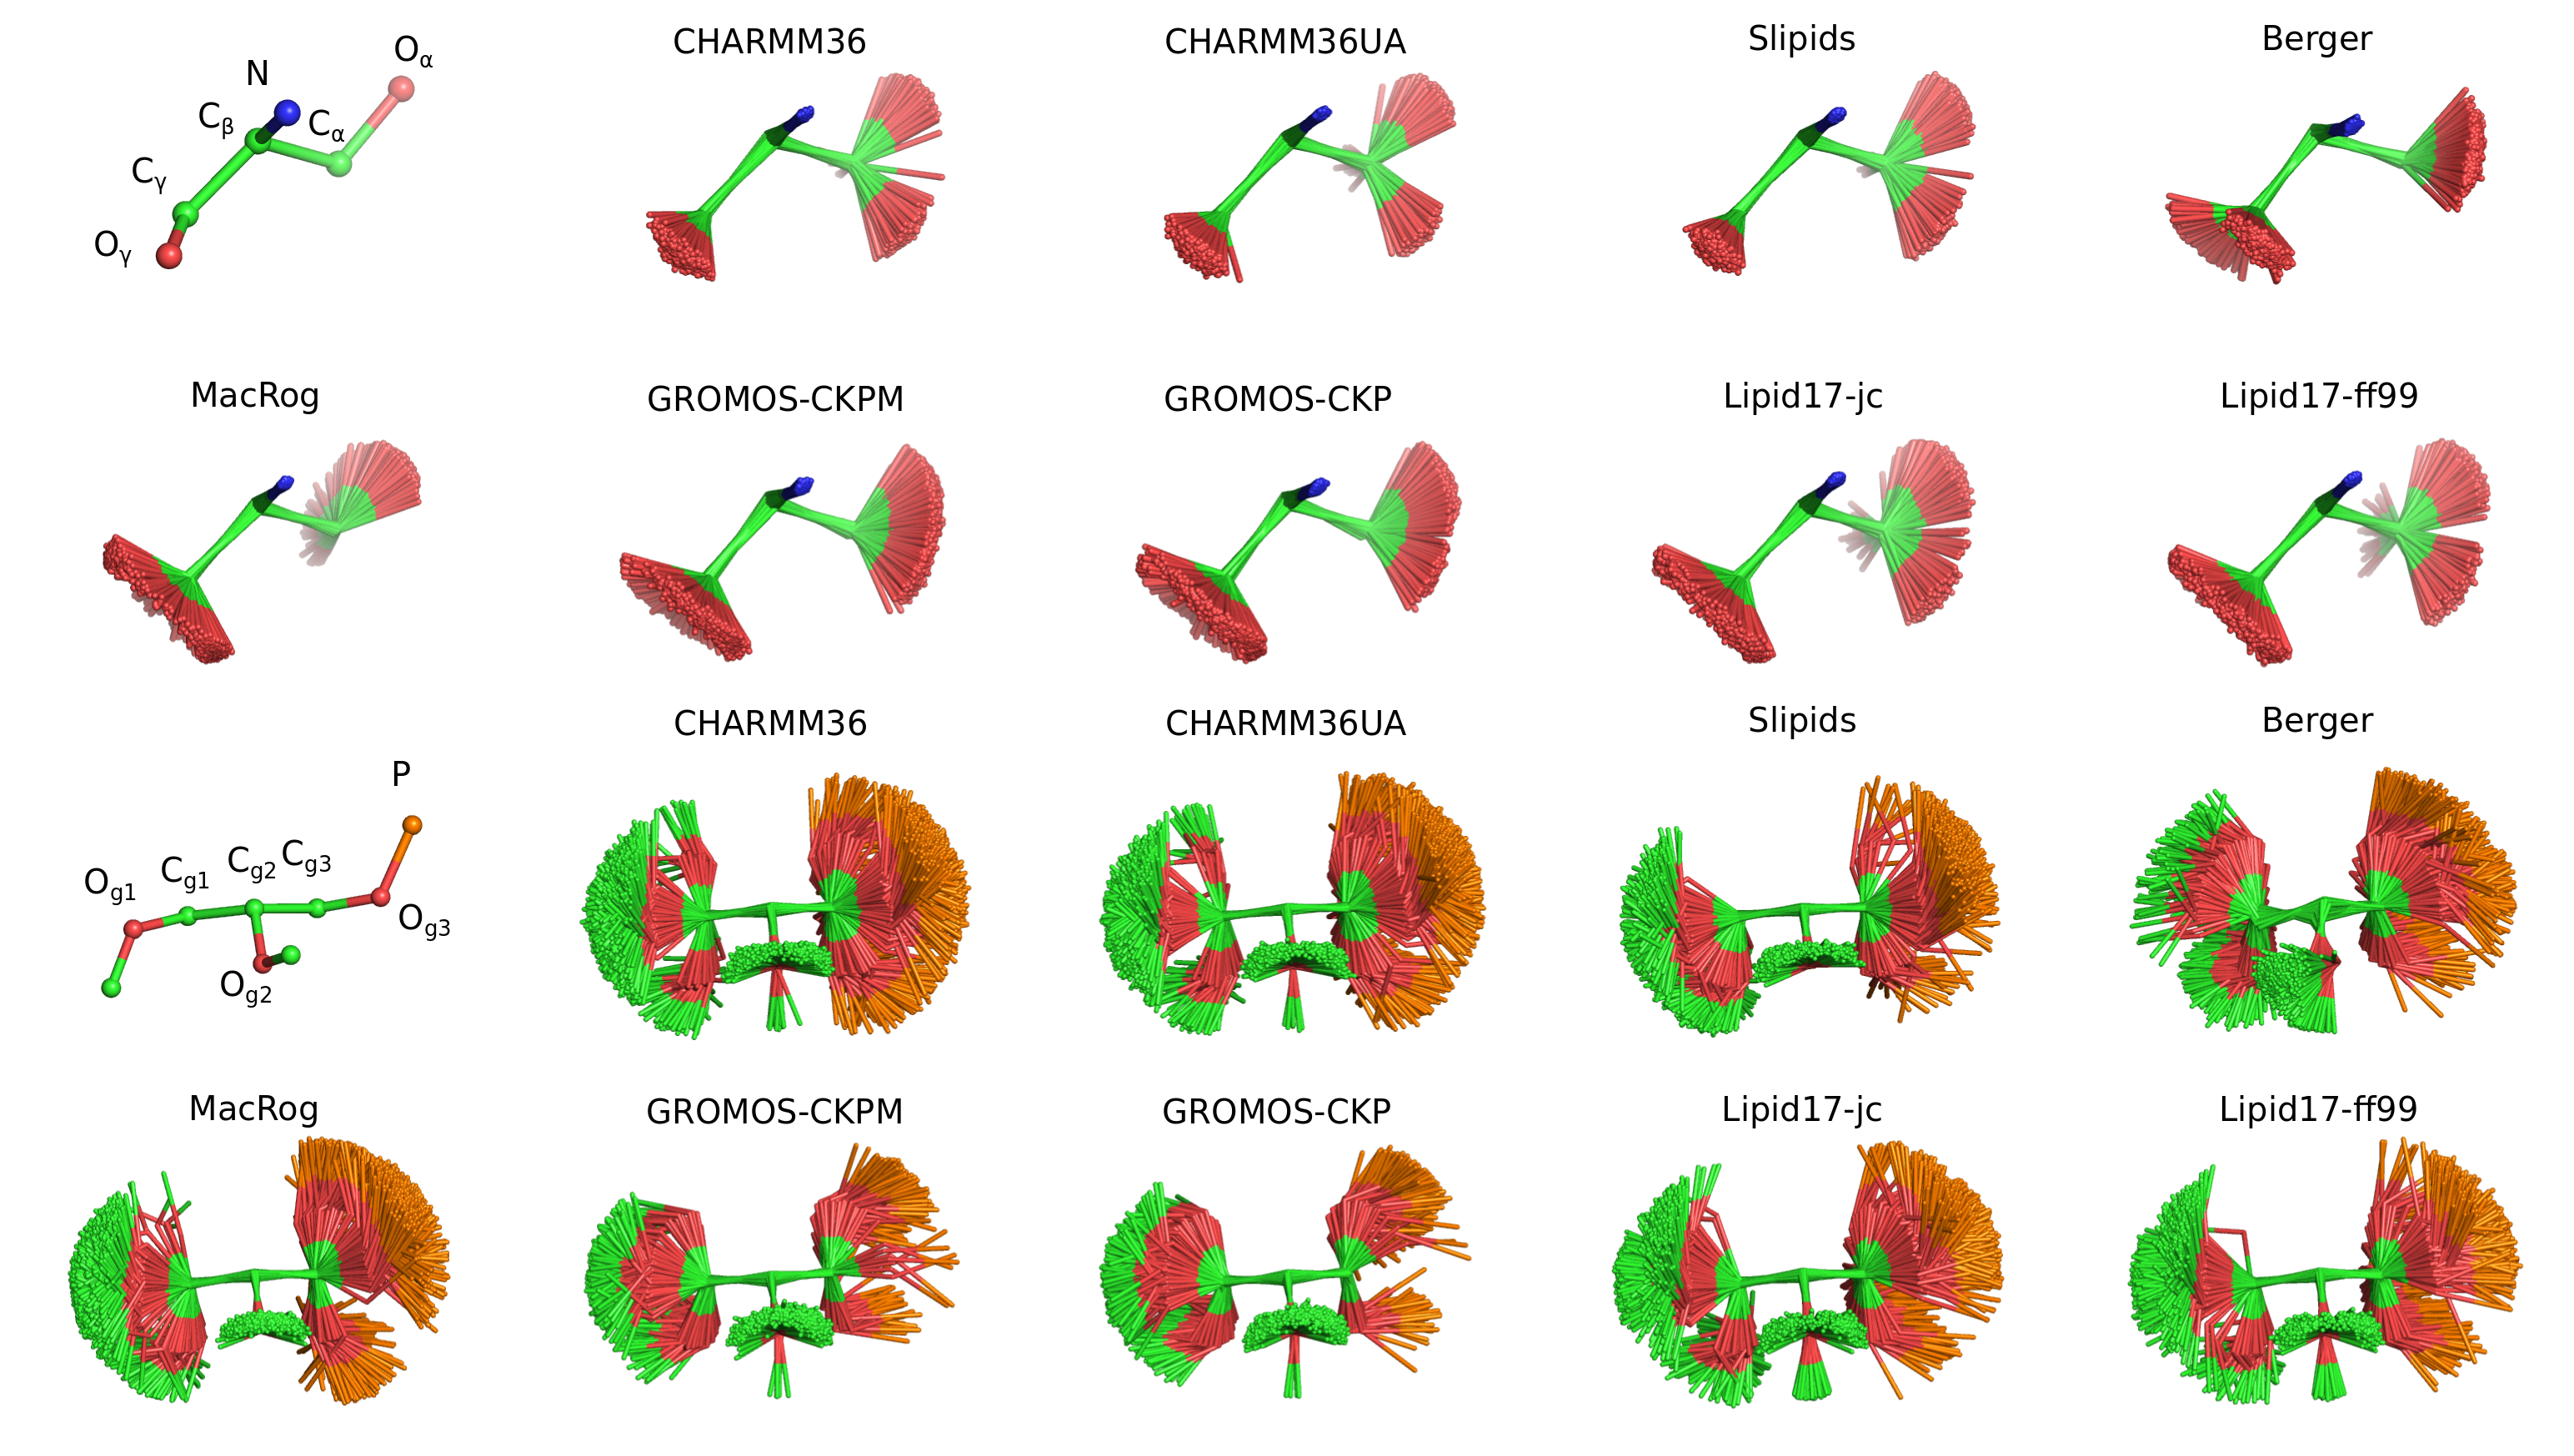
\includegraphics[width=18.0cm]{../Figs/figS8.png}
  \caption{\label{HGandGLYstructuresPS}
    Overlayed snapshots from glycerol backbone and headgroup region from 
    different simulations of PS lipids.
  }
\end{figure*}

\begin{figure*}[]
  \centering
  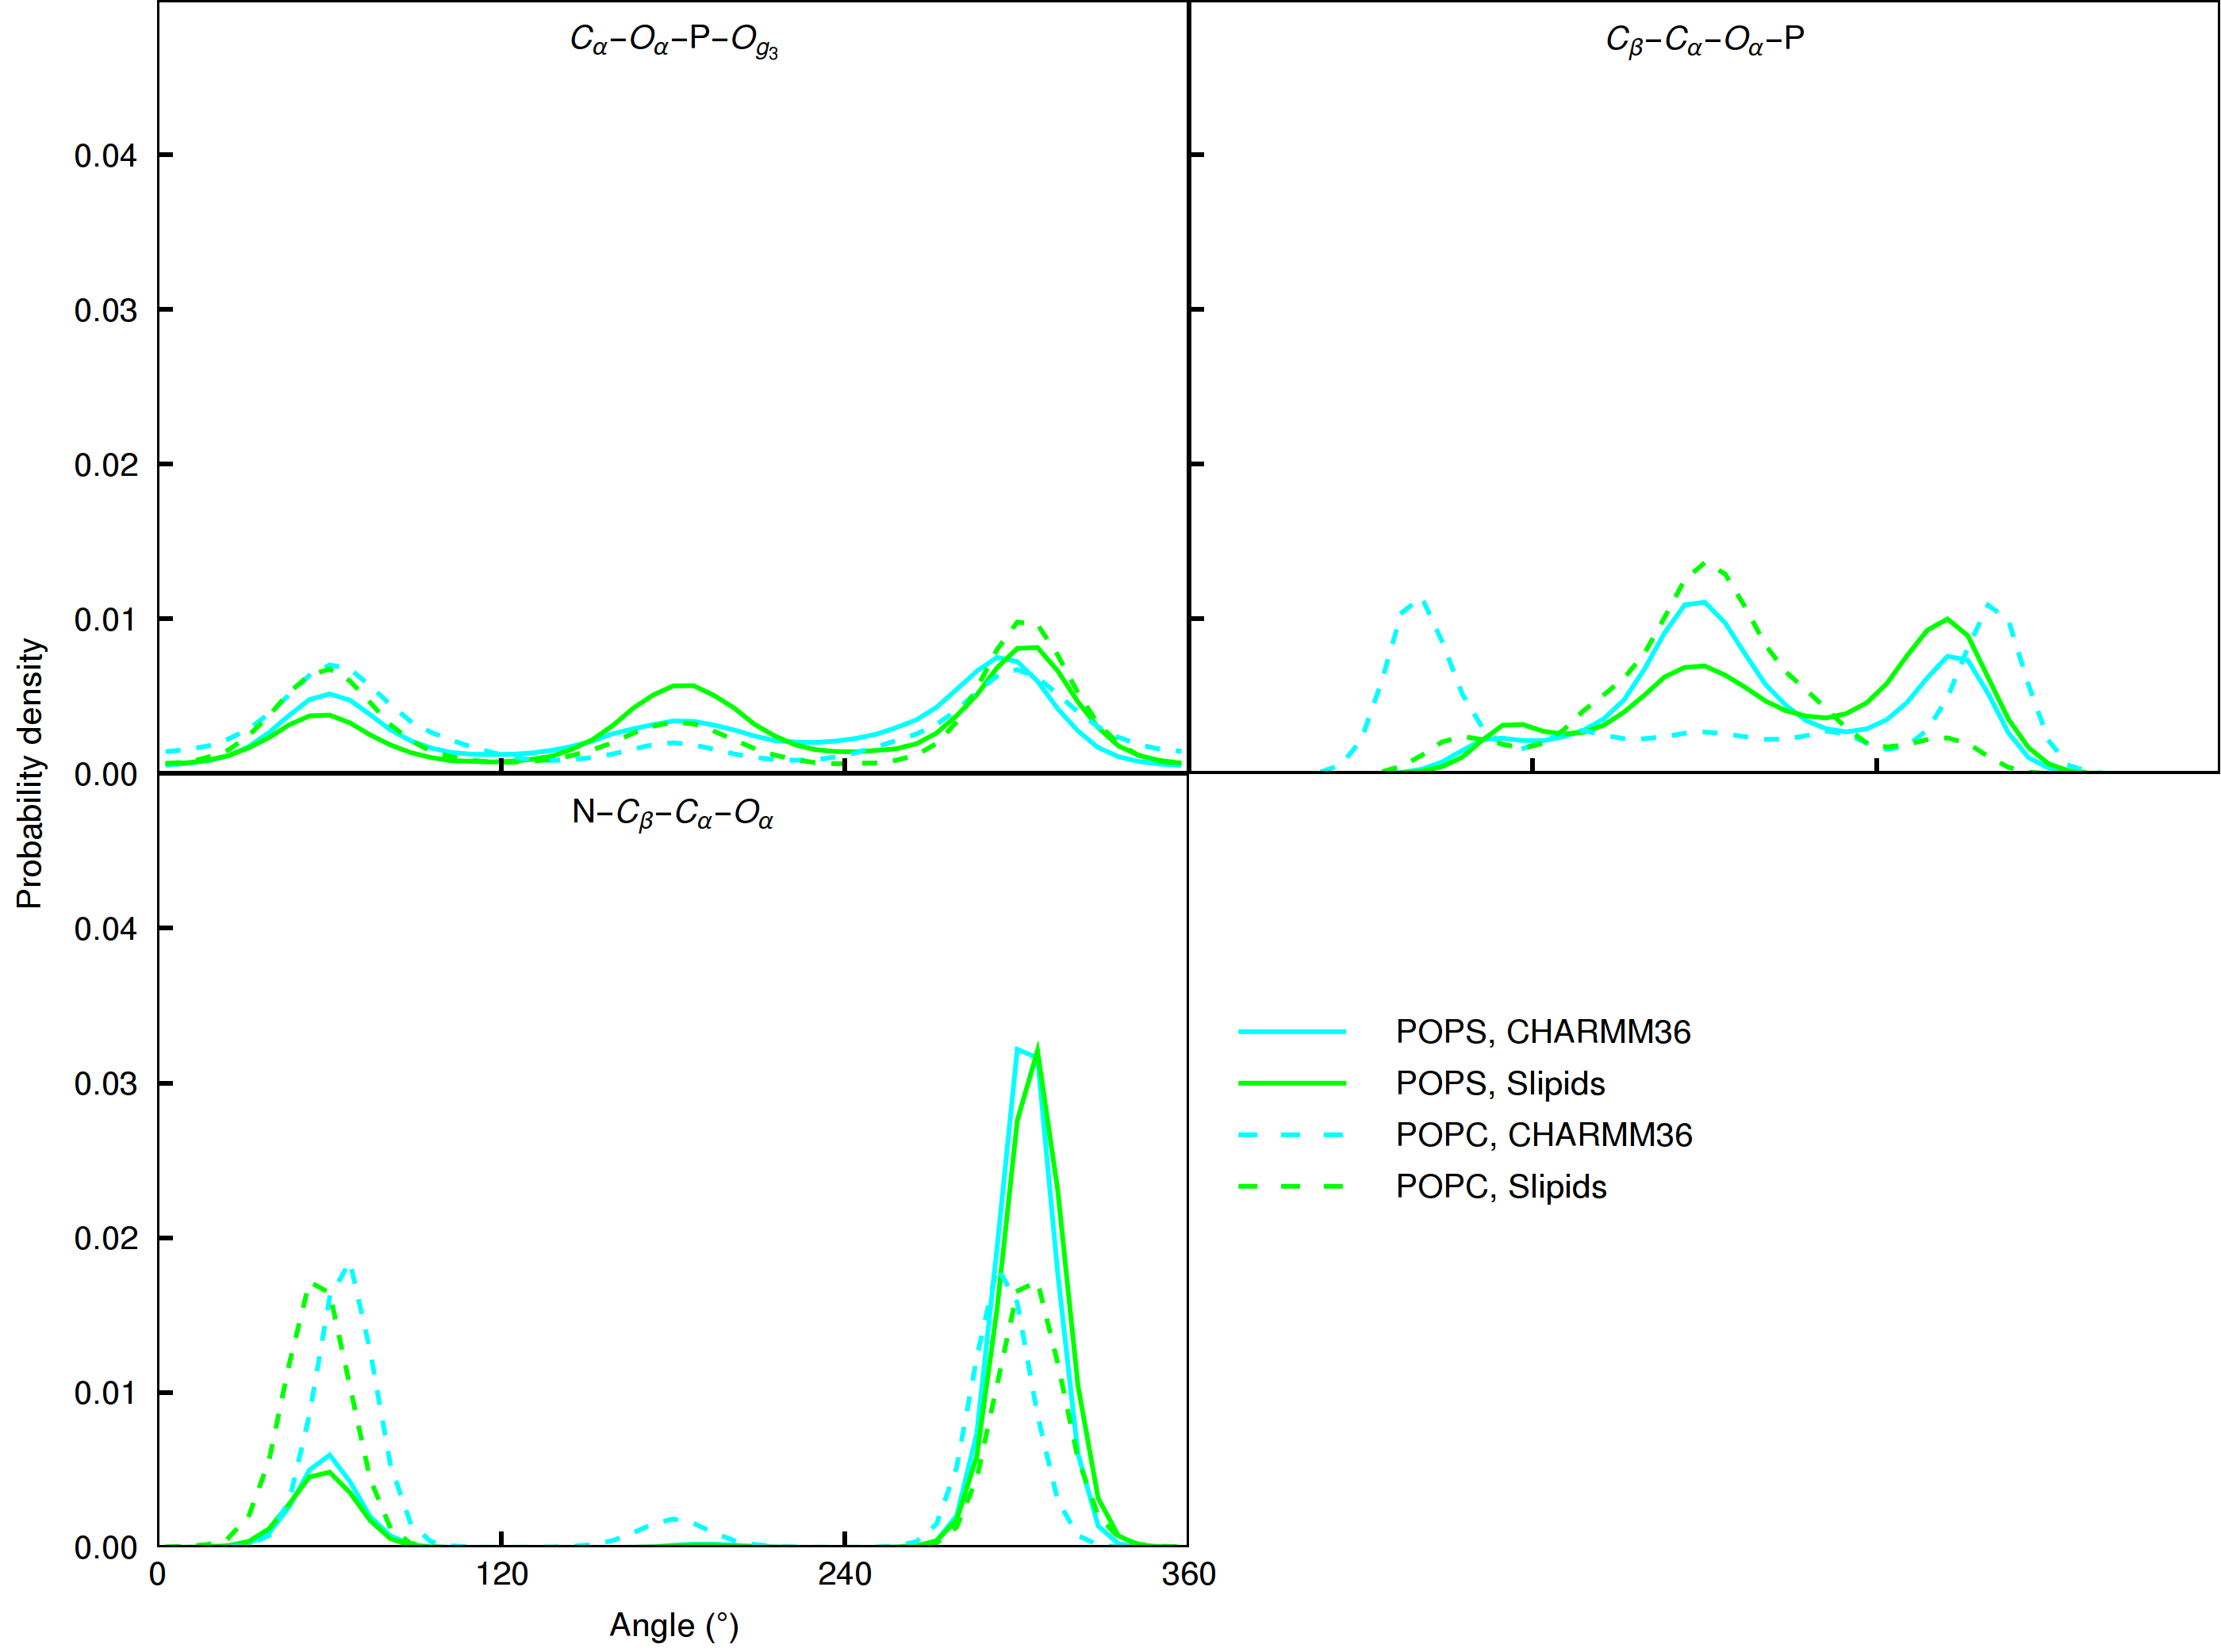
\includegraphics[width=16.0cm]{../Figs/figS7PC.png}
  \caption{\label{dihedralsHGpc}
    Dihedral angle distributions of headgroup region of PS lipids from different simulation models.
  }
\end{figure*}

\begin{figure*}[]
  \centering
  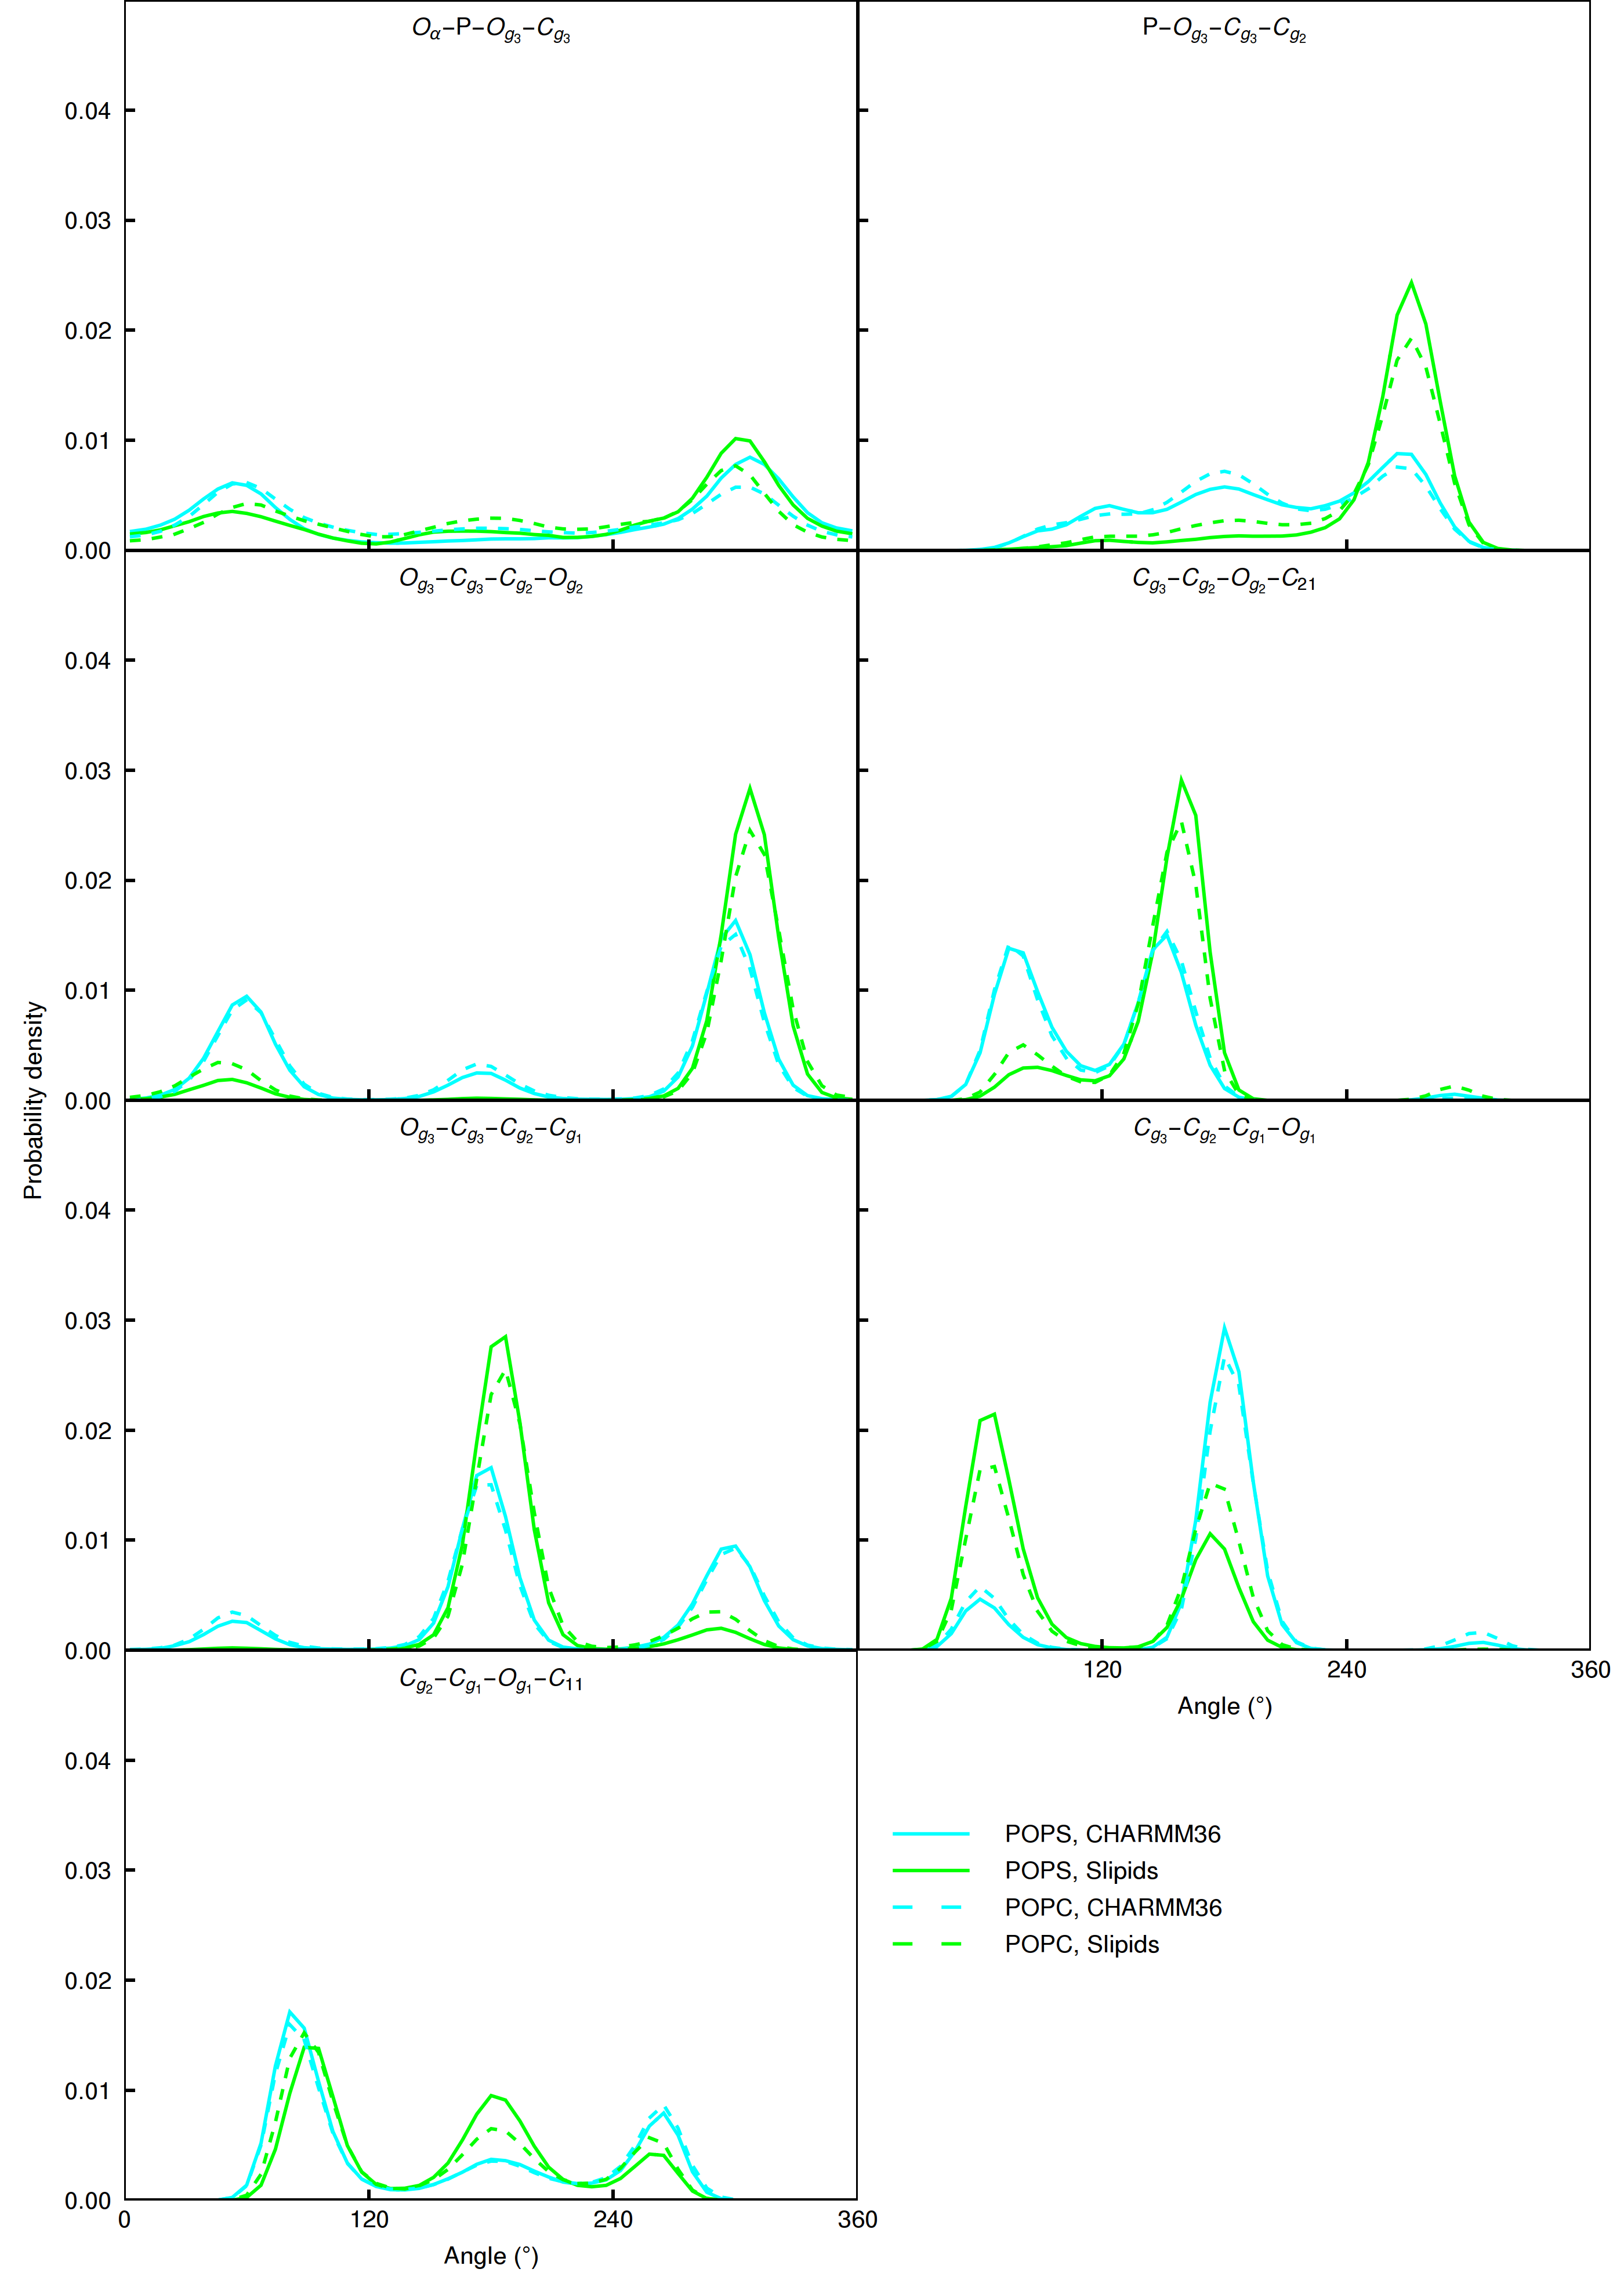
\includegraphics[width=15.0cm]{../Figs/figS6PC.png}
  \caption{\label{dihedralsGLYpc}
    Dihedral angle distributions of glycerol backbone region of PS lipids from different simulation models.
  }
\end{figure*}

\begin{figure}[]
  \centering
  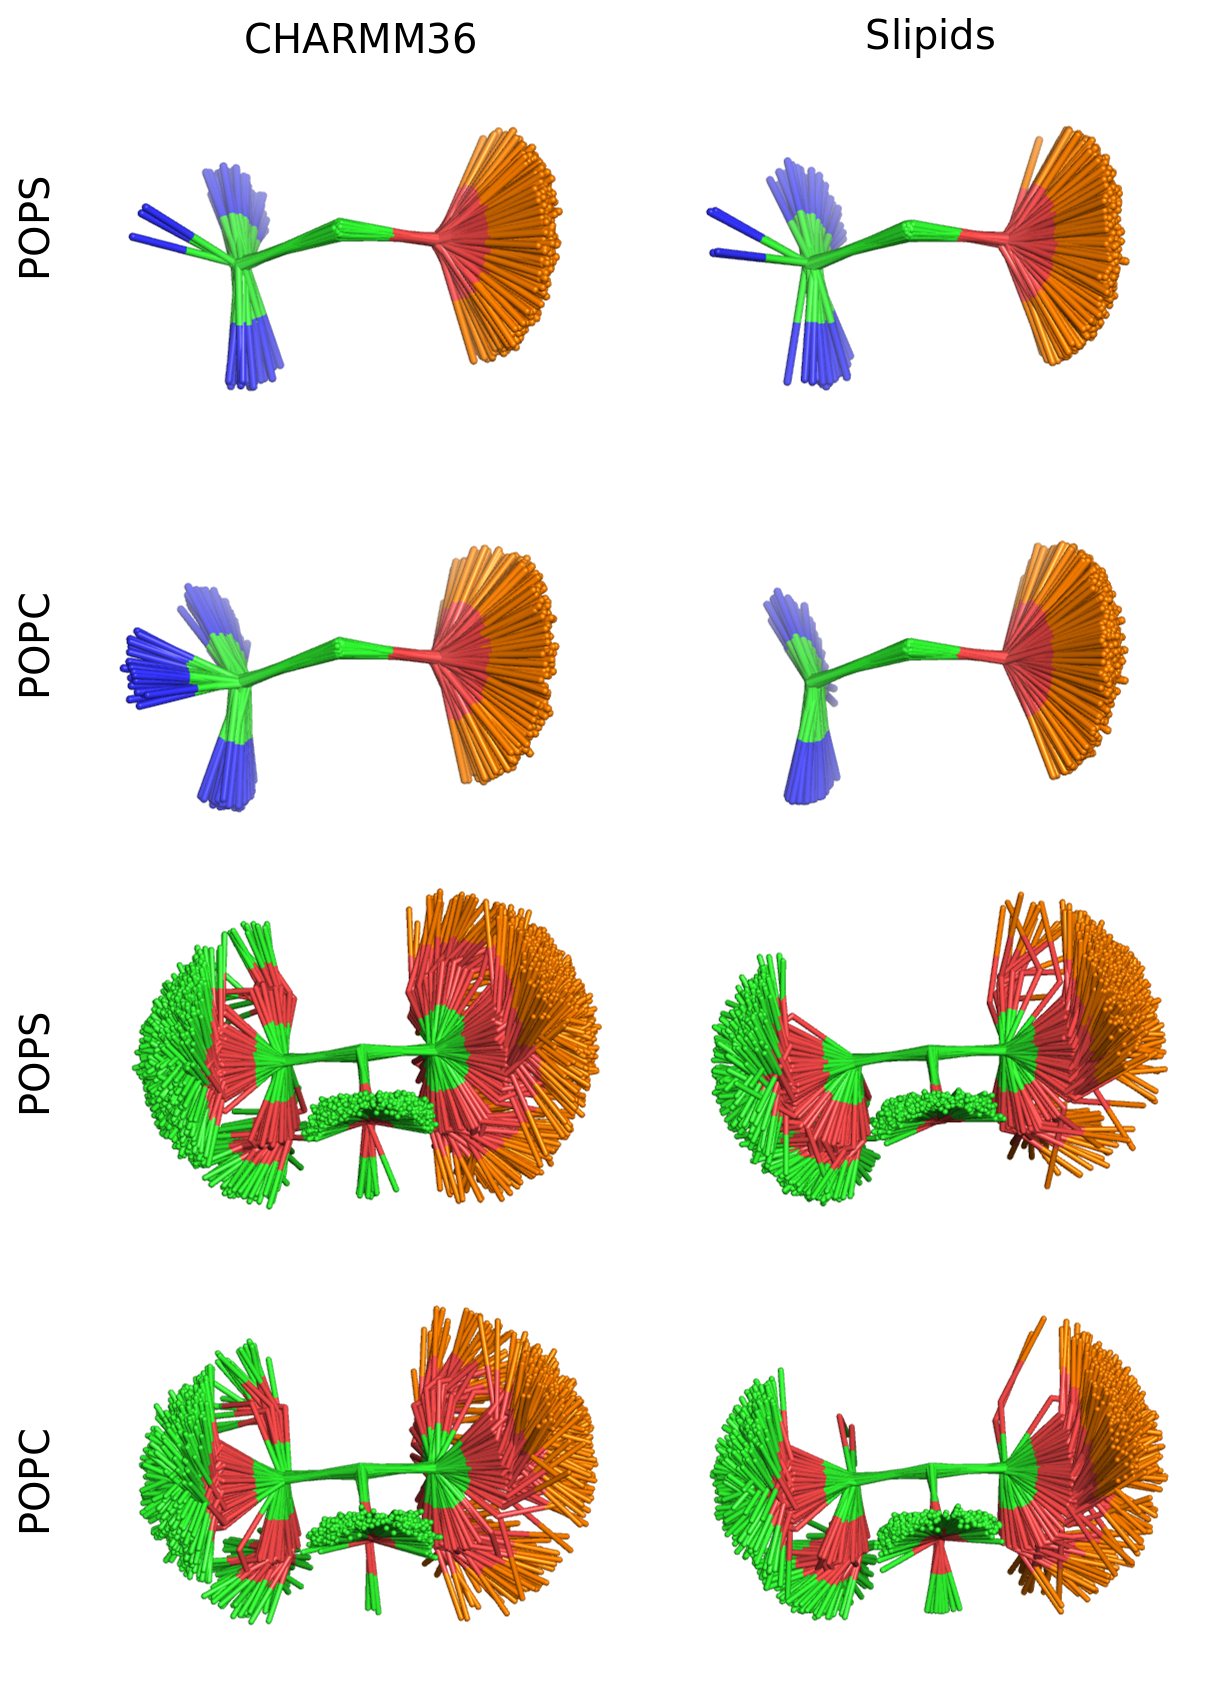
\includegraphics[width=9.0cm]{../Figs/figS8_POPC.png}
  \caption{\label{HGandGLYstructuresPSPC}
    Overlayed snapshots from glycerol backbone and headgroup region from 
    different simulations of PS lipids.
  }
\end{figure}




\pagebreak

\section{Headgroup response to the additional counterions in POPC:POPS (5:1) mixtures}\label{mixtureTOadditionalCIs}
To evaluate counterion binding in different simulation models against experimental data~\cite{roux90},
we plot the headgroup order parameters measured from POPC:POPS 5:1 mixture
as a function of different monovalent ions added to the buffer (Fig. \ref{PSresponseTONaCl}). 
Experimental order parameters of POPC headgroup in the mixture are available as a function
of LiCl and KCl concentrations, while POPS headgroup order parameters are measured also
as a function of NaCl. Lithium interacts more strongly with PS headgroups than other monovalent 
ions~\cite{hauser83,hauser85,roux86,mattai89,roux90}, as also observed for PC headgroups~\cite{cevc90}. 
This is evident also in the changes of PS headgroup order parameters, which decrease with the addition of lithium 
but increase with the addition of sodium or potassium (Fig. \ref{PSresponseTONaCl}). 
POPC headgroup order parameters exhibit a clear decrease as a function of LiCl concentration
but only modest changes as a function of KCl concentration, indicating singificant 
Li$^+$ binding but only weak Na$^+$ binding to the mixture when interpreted using the
electrometer concept~\cite{akutsu81,altenbach84,seelig87}.

In simulations with Berger and CHARMM36 models, the responses of both headgroup order parameter
of POPC and the $\beta$ carbon of POPS to the added sodium or potassium are similar to the experiments
of LiCl (Fig. \ref{PSresponseTONaCl}), indicating overestimated binding affinity of the counterions 
in these simulations. The MacRog simulations with potassium exhibit weaker counterion binding affinity
(Fig. \ref{CIdensPSOCmixt}), but significantly larger error bars and
less systematic changes in the order parameters (Fig. \ref{PSresponseTONaCl}).
Similar unsystematic behaviour was also observed in the simulations of Lipid14/17 model
with the additional counterions \cite{POPCpopsLIPID17withKCI,POPCpopsLIPID17withK,POPCpopsLIPID17withNaCI,POPCpopsLIPID17withNa},
for which the data is not shown due to the formation of
ion clusters in water with relatively low (1 M) ion concentrations (Fig. \ref{ionCLUSTERS}).
Such clusters appering also in MagRog simulations with 4 M concentration of KCl
could explain the unsystematic changes of the order parameters in this model with the added KCl.
In conclusion, the results are in line with the section \ref{ciBINDINGsection}
in the main text, suggesting that the MacRog simulations with KCl give the most
realistic surface charge at the lipid bilayer interface.
\begin{figure*}[]
  \centering
  \includegraphics[width=17.0cm]{../Figs/CHANGESwithMONVALENTwithPS.eps}
  \caption{\label{PSresponseTONaCl}
    Changes of the PC (left) and PS (right) headgroup order parameters as a function of
    added NaCl, KCl and LiCl from POPC:POPS (5:1) mixture at 298~K
    (except Berger simulations are (4:1) mixture at 310~K).
    The experimental data is from Ref. \citenum{roux90}.
    The values from counterion-only systems are set as a zero point of y-axis.
    To correctly illustrate the significant forking of the $\alpha$-carbon order parameter
    in PS headgroup (bottom, right), the y-axis is tranferred with the same value for both order parameters such that the lower order
    parameter value is at zero.
  }
\end{figure*}
\begin{figure}[]
  \centering
  \includegraphics[width=8.0cm]{../Figs/CIdensPSOCmixt.eps}
  \caption{  Counterion density distributions from PC:PS mixtures.
\label{CIdensPSOCmixt}
  }
\end{figure}
\begin{figure}[]
  \centering
  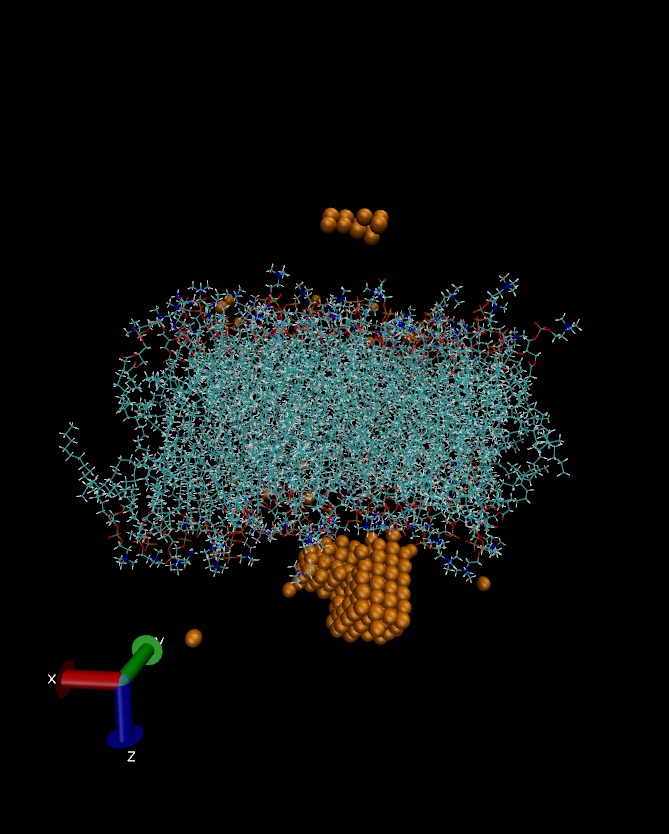
\includegraphics[width=8.0cm]{../Figs/lipid17cluster.png}
  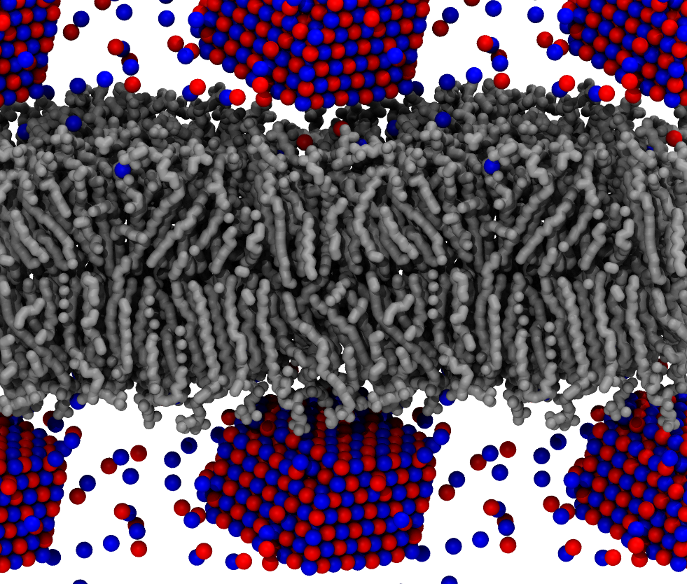
\includegraphics[width=8.0cm]{../Figs/MacRogIONcluster.png}
  \caption{Ion clusters appearing in POPC:POPS (5:1) lipid17/14 simulations with 1 M of NaCl (left)
    and MacRog simulations with 4 M of KCl (right).
\label{ionCLUSTERS}
  }
\end{figure}
\newpage


%%
%% I think that this section is not very useful, I think that we should remove it.
%%
%\section{Sodium binding to DMPC:DOPS mixture}
%
%\begin{figure}[]
%  \centering
%  \includegraphics[width=9.0cm]{../Figs/PSresponseTONaCl.eps}
%  \caption{\label{PSresponseTONaClDMPC}
%    Order parameters of PS headgroup as a function of added NaCl measured from DMPC:DMPS (3:1) mixture \cite{roux86}.
%  }
%\end{figure}
%The experimental results show essentially no changes in the order parameters as a function of
%added NaCl, while significant changes are observed in simulations. However,
%the minimum buffer concentration of NaCl in the experimental was 100mM \cite{roux86}.
%Therefore, we cannot exclude the possibility that the NaCl induced changes were already
%saturated with 100mM NaCl concentration, which was the case for CaCl$_2$ in Fig. \ref{changesWITHCaClPS}.



\section{Calcium binding to POPC in CHARMM36 simulation with NBfix}\label{CHARMMcalciumNBfix}

The response of POPC headgroup order parameters to the CaCl$_2$ concentration
are underestimated in simulations of POPC:POPS (5:1) mixture with CHARMM36 containing
the NBfix for interactions between calicum and lipid oxygens \cite{kim16}
(Fig. \ref{changesWITHCaClPS} in the main text),
indicating that the calcium binding to the bilayer is too weak with these
parameters. Without the NBfix term, the calcium binding affinity to pure POPC
lipid bilayers was overestimated in the CHARMM36 model \cite{catte16}.
However, after employing the NBfix term, the response of headgroup order
parameters (Fig. \ref{OP_CHARMM_CaCl_POPC_NBFix}) and the binding affinity
(Fig. \ref{density_profile_CHARMM_CaCl_POPC_NBFix}) of calcium also to a pure
POPC bilayer are underestimated. Notably, CHARMM36 simulations with the NBfix
terms \cite{venable13,kim16} employed predict similar binding affinity for sodium and calcium.
In conclusion, the special NBfix~\cite{kim16} for calcium, 
incorporated in the parameters give by the CHARMM-GUI at the time
of running the simulations (January 2018), leads to the underestimation of
calcium binding affinity to pure PC and mixed PC:PS bilayers.

\begin{figure}[]
  \centering
  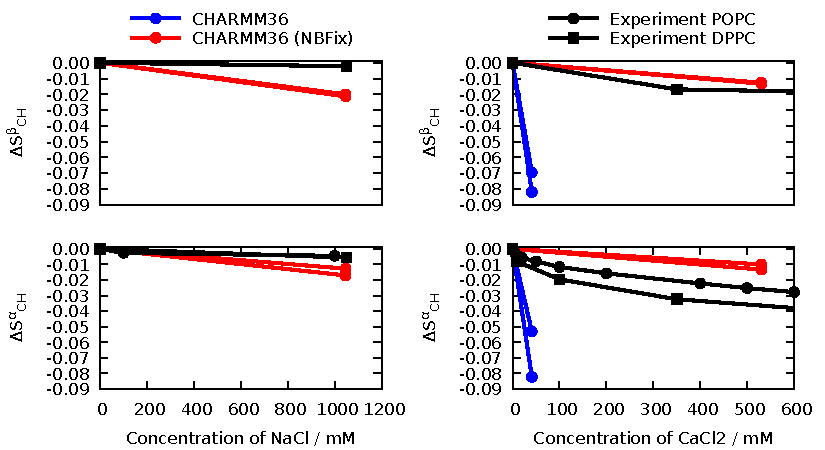
\includegraphics[width=17.0cm]{../Figs/OP_CHARMM_CaCl_POPC_NBFix.pdf}
  \caption{\label{OP_CHARMM_CaCl_POPC_NBFix}
    Headgroup order parameters from CHARMM36 simulations of POPC mixed with ions having
    the NBfix term employed for sodium \cite{venable13} ({\it left})
    and calcium \cite{kim16} ({\it right}) compared with the experimental data \cite{akutsu81,altenbach84}
    and simulations without NBfix for the calcium.
    Simulation files without ions are available at Ref. \citenum{nencineCHARMM36popcT310K},
    with the NBfix term in sodium at Ref. \citenum{CHARMM36withCaClNBfix}, 
    with the NBfix term in calcium at Ref. \citenum{CHARMM36withCaClNBfix} and
    without the NBfix in calcium at Ref. \citenum{charmmPOPC450mMCaClfiles}.
  }
\end{figure}

\begin{figure}[]
  \centering
  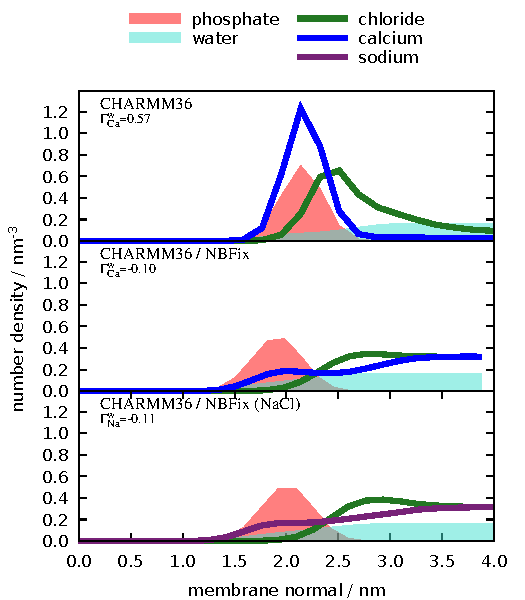
\includegraphics[width=9.0cm]{../Figs/density_profile_CHARMM_CaCl_POPC_NBFix.pdf}
  \caption{\label{density_profile_CHARMM_CaCl_POPC_NBFix}
    Density profiles along membrane normal from CHARMM36 simulations with (middle)
    and without (top) the NBfix term for calcium \cite{kim16} compared to the simulation
    with the NBfix term for sodium \cite{venable13} (bottom). The simulation data are the same as in figure \ref{OP_CHARMM_CaCl_POPC_NBFix}.
  }
\end{figure}

\pagebreak
\section{Calcium density profiles from simulations with POPC:POPS(5:1) mixture}
\begin{figure}[ht]
  \centering
  \includegraphics[width=9cm]{../Figs/CAdensPCPSmixture.eps}
  \caption{\label{CAdensPCPSmixtureALL}
    Ca2+ density profiles from simulations.
  }
  \todo{The CHARMM results are mass densities, number densities should be used when the data by Jesper Madsen is available.} \\
  \todo{Should we include also counterions into the plot?} \\
\end{figure}

\pagebreak
\section{Details of the rough subjective force field ranking (Fig.~\ref{comparisonTablePS})} 

The assessment was based fully on the Fig.~\ref{HGorderParametersPS}.
%
First, for each carbon (the columns in Fig.~\ref{HGorderParametersPS}) in each force field (the rows),
we looked separately at deviations in magnitude and forking.

{\bf Magnitude} deviations, i.e., how close to the experimentally obtained C--H order parameters (OPs)
the force-field-produced OPs were.
%
For each carbon, the following 5-step scale was used:
%
\begin{description}
\item [0 (~):] \noindent {More than half of all the calculated OPs (that is, of all different hydrogens in all different lipids) were within the {\it subjective sweet spots} (SSP, blue-shaded areas in Fig.~\ref{HGorderParametersPS}).}
%
\item [1 ({\textsf{\tiny M}}):] \noindent {All the calculated OPs  were $< 0.03$ units away from the SSP.}
%
\item [2  ({\textsf{\small M}}):] \noindent {All the calculated OPs  were $< 0.05$ units away from the SSP.}
%
\item [3 ({\textsf{\large M}}):] \noindent {All the calculated OPs  were $< 0.10$ units away from the SSP.}
%
\item [4 ({\textsf{\Large M}}):] \noindent {Some of the calculated OPs  were $> 0.10$ units  away from the SSP.}
\end{description}

{\bf Forking} deviations, i.e., how well the difference in order parameters of two hydrogens attached to a given carbon matched that obtained experimentally. Note that this is not relevant for $\beta$ and $\mathrm{g_2}$, which have only one hydrogen. For the $\alpha$ carbon,  for which a considerable forking of 0.105 is experimentally seen, the following 5-step scale was used:
\begin{description}
\item [0 (~):] \noindent {The distance $D$ between the dots (that mark the measurement-time-weighted averages in Fig.~\ref{HGorderParametersPS}) was $0.08 < D< 0.13$ units for all the calculated OPs (that is, for all different lipids).}
%
\item [1 ({\textsf{\tiny F}}):] \noindent {$(0.06 < D < 0.08)$ OR $(0.13 < D < 0.15)$.}
%
\item [2  ({\textsf{\small F}}):] \noindent {$(0.04 < D < 0.06)$ OR $(0.15 < D < 0.17)$.}
%
\item [3 ({\textsf{\large F}}):] \noindent {$(0.02 < D < 0.04)$ OR $(0.17 < D < 0.19)$.}
%
\item [4 ({\textsf{\Large F}}):] \noindent {$(D<0.02)$ OR $(0.19<D)$.}
\end{description}
%
For the $\mathrm{g_3}$ carbon, for which no forking is indicated by experiments, the following 5-step scale was used:
%
\begin{description}
\item [0 (~):] \noindent {$ D< 0.02$.}
%
\item [1 ({\textsf{\tiny F}}):] \noindent {$0.02 < D < 0.04$.}
%
\item [2  ({\textsf{\small F}}):] \noindent {$0.04 < D < 0.06$.}
%
\item [3 ({\textsf{\large F}}):] \noindent {$0.06 < D < 0.08$.}
%
\item [4 ({\textsf{\Large F}}):] \noindent {$0.08 < D$.}
\end{description}
%
For the $\mathrm{g_1}$ carbon, for which a considerable forking of 0.13 is experimentally seen, the following 5-step scale was used:
%
\begin{description}
\item [0 (~):] \noindent {$0.11 < D < 0.15$.}
%
\item [1 ({\textsf{\tiny F}}):] \noindent {$(0.09 < D < 0.11)$ OR $(0.15 < D < 0.17)$.}
%
\item [2  ({\textsf{\small F}}):] \noindent {$(0.07 < D < 0.09)$ OR $(0.17 < D < 0.19)$.}
%
\item [3 ({\textsf{\large F}}):] \noindent {$(0.05 < D < 0.07)$ OR $(0.19 < D < 0.21)$.}
%
\item [4 ({\textsf{\Large F}}):] \noindent {$(D<0.05)$ OR $(0.21<D)$.}
\end{description}

Based on these assessments of magnitude and forking deviations,
each carbon was then assigned to one of the following groups:
"within experimental error"
(magnitude and forking deviations both on step 0 of the scales described above),
"almost within experimental error"
(sum of the magnitude and forking deviation steps 1 or 2),
"clear deviation from experiments"
(sum of magnitude and forking deviation steps from 3 to 5), and
"major deviation from experiments"
(sum of magnitude and forking deviation steps from 6 to 8).
These groups are indicated by colors in Fig.~4.
(Note that for $\beta$ and $\mathrm{g_2}$, for which there can be no forking,
the corresponding group assigment limits were: 0, 1, 2, and 3.)

Finally, the total ability of the force field to describe the headgroup and
glycerol structure was estimated.
To this end, the groups were given the following weights:
0 (within experimental error),
1 (almost within experimental error),
2 (clear deviation from experiments),
4 (major deviation from experiments),
and the weights of the five carbons were summed up.
The sum, given in the $\Sigma$-column of Fig.~\ref{HGorderParametersPS},
was then used to (roughly and subjectively, as should be clear from the
above description) rank the force fields.



\newpage
\bibliography{refs.bib}

\end{document}
